\definecolor{gold}{rgb}{0.77,0.69,0.37}
\newlength{\hptitlewidth}
\newlength{\rationalh}
\newcommand{\hptitle}[2][\stockwidth]{%
  \setlength{\hptitlewidth}{#1}%
  \centering\color{white}%
  \vskip 3cm\resizebox{.95\hptitlewidth}{!}{\textls[100]{HARRY POTTER AND THE}}%
  \vskip 2mm%
  \color{gold}%
  \settoheight{\rationalh}{\resizebox{.95\hptitlewidth}{!}{\textls[20]{RATIONALITY}}}
  \resizebox{!}{\rationalh}{\textls[50]{METHODS}}%
  \hfil\resizebox{!}{\rationalh}{\textls[50]{OF}}%
  \vskip 2mm%
  \resizebox{.95\hptitlewidth}{!}{\textls[20]{RATIONALITY}}%
  \vskip 8mm%
  \color{white}%
  \resizebox{.5\hptitlewidth}{!}{\textls[50]{\scshape{}by Eliezer Yudkowsky}}%
  \vfill%
  \textls[50]{\scshape #2}%
  \color{black}%
  \vskip 1cm\ %
}
\providecommand{\fullvolumetitle}[1]{Book #1: \volumetitle}

\ifcover%
\newpagecolor{black}\afterpage{\restorepagecolor}
\newcommand\BackgroundPic{
\put(0,0){%
\parbox[b][\paperheight]{\paperwidth}{%
\vfill%
\centering%
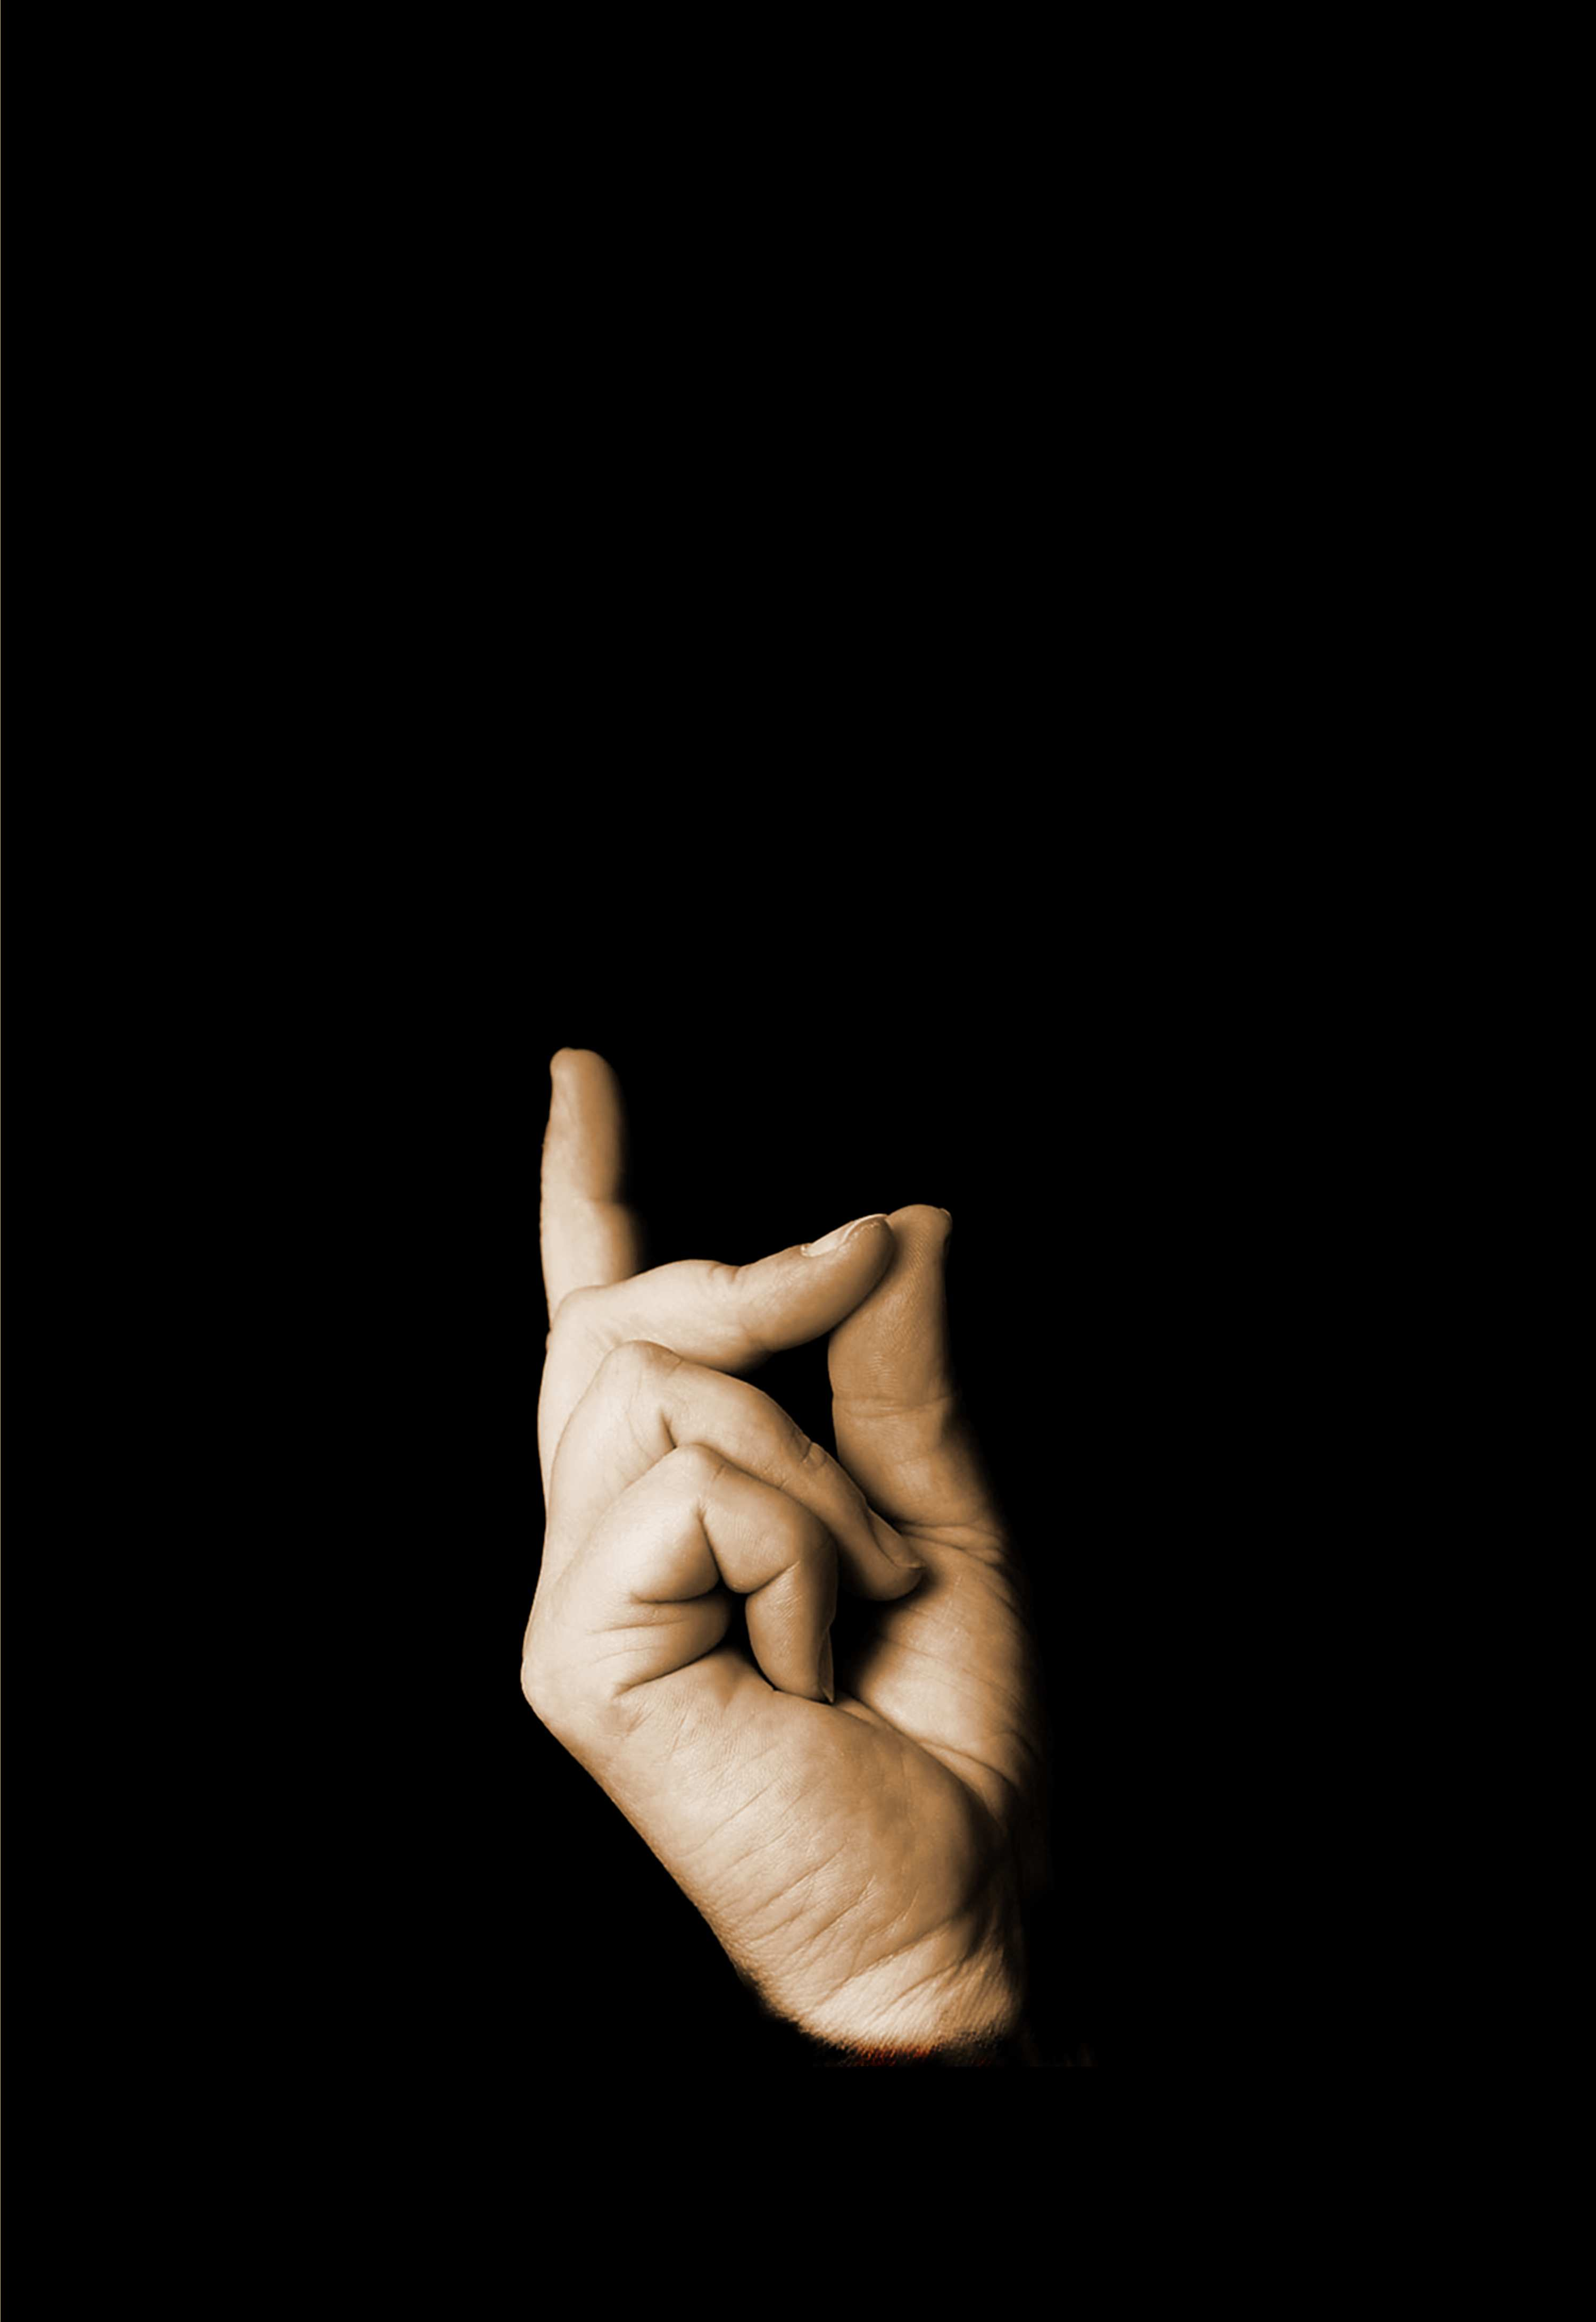
\includegraphics[width=\paperwidth,height=\paperheight,keepaspectratio]{images/cover0.jpg}%
\vfill%
}}}\AddToShipoutPicture*{\BackgroundPic}%
\AddToShipoutPicture*{\put(0,0){%
\parbox[b][\paperheight]{\paperwidth}{%
\hptitle{\fullvolumetitle{\volumenumber}}%
}}}%
\ %
\cleartorecto
\fi
\begin{center}
\thispagestyle{empty}
{\hpfont
\Huge\MakeUppercase{Harry Potter}\vspace*{0.5cm}

\Large\MakeUppercase{and the Methods of Rationality} %

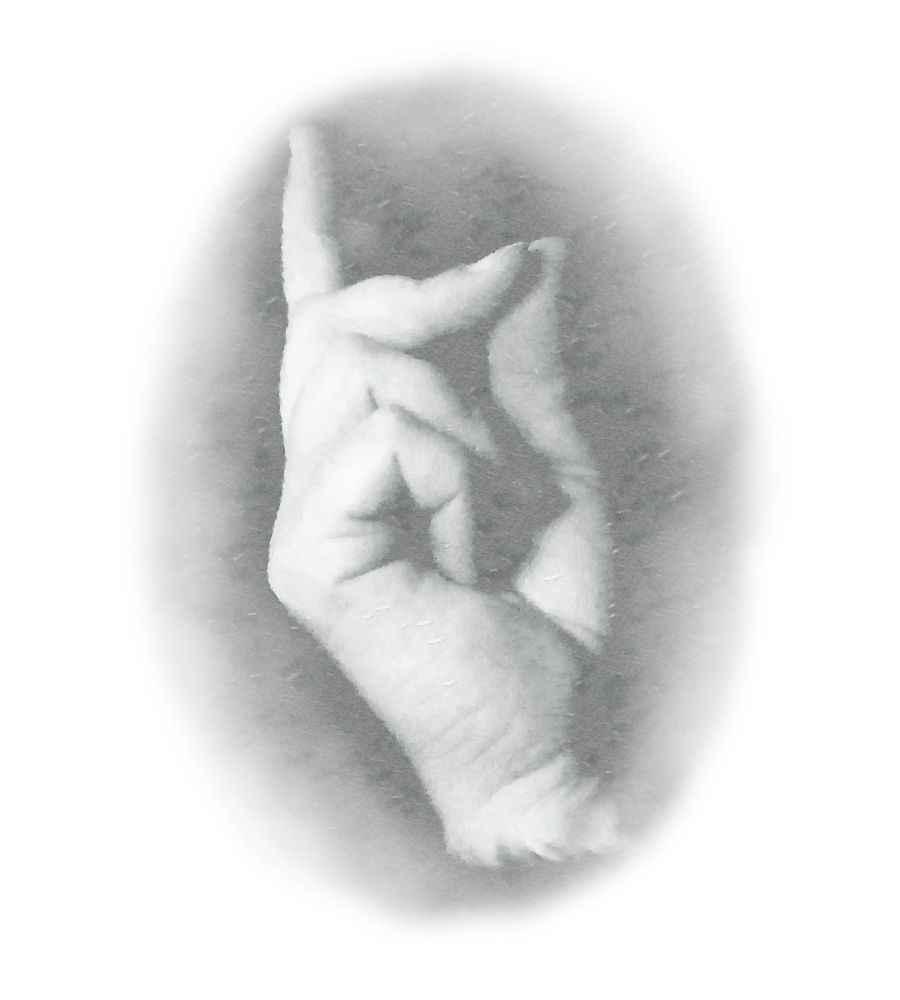
\includegraphics[scale=0.5]{images/bubble0.jpg}

\Large BY \vspace*{.25cm}

\huge \MakeUppercase{Eliezer Yudkowsky}%

\normalsize

\vspace*{1\baselineskip}
\fullvolumetitle{\volumenumber}
}

\vfill
Find the original text, with author's notes, fan art and other info at:\\
\url{http://hpmor.com}

Home of this revised e-book version is:\\
\url{https://github.com/rrthomas/hpmor/}
\end{center}

\cleartoverso

\begin{center}
\vspace*{2cm}

\thispagestyle{empty}
Fanfiction based on the characters of

\vspace*{.5cm}

\Large \MakeUppercase{J.~K.~Rowling} \normalsize

\vspace*{.5cm}

and her books:

\vspace*{.5cm}

{
        \newcounter{books_list_counter}
        \def \hpBook #1{
                \addtocounter{books_list_counter}{1}
                \textit{Harry Potter and the #1} \par
                Year \numtoName{\value{books_list_counter}} at Hogwarts
                \smallskip\par
        }
        \hpBook{Philosopher's Stone}
        \hpBook{Chamber of Secrets}
        \hpBook{Prisoner of Azkaban}
        \hpBook{Goblet of Fire}
        \hpBook{Order of the Phoenix}
        \hpBook{Half-Blood Prince}
        \hpBook{Deathly Hallows}
}
\end{center}
\cleartorecto% FIXME: For some reason, without this the contents ends up on a verso page (an extra blank page is added)

% \chapter{Disclaimer}
\newpage
\vspace*{4cm}
\begin{center}
Disclaimer:\\J.~K.~Rowling owns Harry Potter,\\and no-one owns the methods of rationality.
\end{center}

\vfill
This e-book was created at \today{}.
